%---------------------------------------------------------------------------------------------------------
%---------------------------------------------------------------------------------------------------------
\section{Pr\'esentation de \hampath}

\subsection{Introduction}

Le code \hampath\ est d\'evelopp\'e par J.-B.~Caillau, Prof. \`a l'Institut de Math\'ematiques de Bourgogne (Dijon), O.~Cots et J.~Gergaud.
Ce code permet~:
\begin{itemize}
    \item de r\'esoudre les probl\`emes de contr\^ole optimal \`a commandes continues via la m\'ethode du tir simple~;
    \item de r\'esoudre les probl\`emes de contr\^ole optimal \`a commandes non continues via la m\'ethode du tir multiple~;
    \item de r\'esoudre les familles de probl\`emes de contr\^ole optimal \`a un param\`etre via la m\'ethode homotopique (hors programme)~;
    \item de calculer les conditions du deuxi\`eme ordre via les points conjugu\'es (hors programme).
\end{itemize}

\subsection{Sch\'ema g\'en\'eral de \hampath}

L'utilisateur fournit \`a \hampath\ en \fortran\ la fonction de tir $S(y)$ et le hamiltonien maximis\'e $h(z) \coloneqq \max_u H(z,p^0,u)$,
et apr\`es compilation de ces routines, \hampath\ fournit une liste de fonctions \matlab~: \cmd{hfun}, \cmd{hvfun}, \cmd{exphvfun}, \cmd{dhvfun}, \cmd{expdhvfun},
\cmd{sfun}, \cmd{sjac}, \cmd{ssolve}, \cmd{hampath}\ldots

\begin{figure}[ht!]
    \begin{center}
        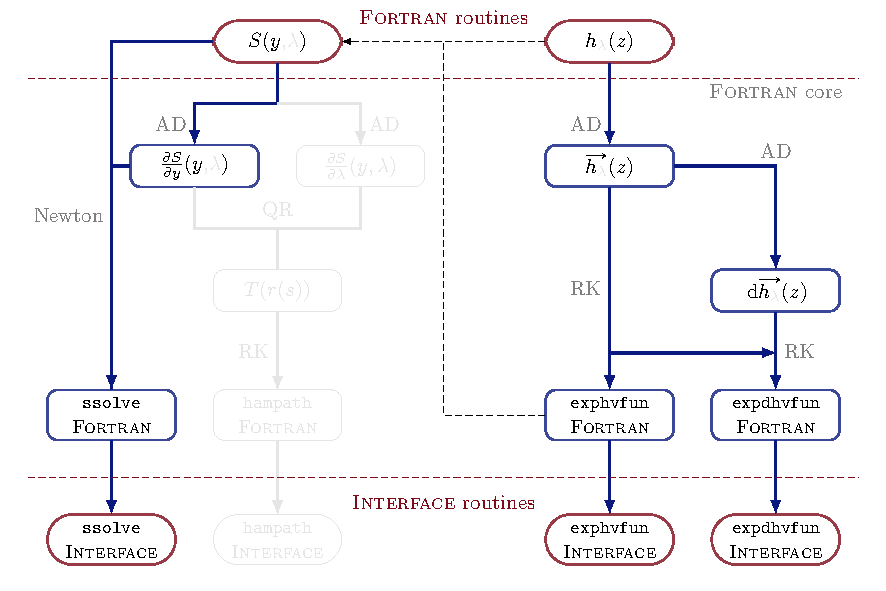
\includegraphics[width=0.72\textwidth]{schemaSimplifie}
    \end{center}
    \caption{Vue sch\'ematique de \hampath.}
    \label{fig:schemaSimplifie}
\end{figure}

%---------------------------------------------------------------------------------------------------------
%---------------------------------------------------------------------------------------------------------
\section{Tir simple et \hampath}

\subsection{Exemple}

Consid\'erons l'exemple de tir simple de la documentation (disponible sous Moodle) de \hampath~:
\vspace{-1em}
\leqnomode
\begin{equation}\label{eq:pbsimple}
    \tagProblem
    \left\{
    \begin{array}{l}
        \displaystyle J(u(\cdot)) = \frac{1}{2} \int_{t_0}^{t_f}u(t)^2 \diff t \longrightarrow \min                             \\[1.0em]
        \displaystyle \dot{x}(t) = v(t),                                                                                        \\
        \displaystyle \dot{v}(t) = -\lambda v(t)^2+u(t), \quad u(t) \in \R, \quad t \in \intervalleff{t_0}{t_f} \text{ p.p.},   \\[1.0em]
        \displaystyle x(t_0) = x_0,   \quad x(t_f) = x_f,                                                                       \\
        \displaystyle v(t_0) = v_0,   \quad v(t_f) = v_f,
    \end{array} 
    \right.
\end{equation}
\reqnomode
avec $t_0 = 0$, $t_f = 1$, $q_0 \coloneqq (x_0,v_0) = (-1,0)$ et $q_f \coloneqq (x_f,v_f) = (0,0)$. On d\'efinit le vecteur de param\`etres
$par \coloneqq (t_0, t_f, x_0, v_0, x_f, v_f, \lambda)$.

\subsubsection{Impl\'ementation par l'utilisateur de la routine \fortran\ \cmd{hfun}}

\begin{myremark}
    La variable \vrb{iarc} a le m\^eme r\^ole que lors des TP sous \matlab\ !
\end{myremark}

Le PMP nous donne le contr\^ole optimal (cf.\ listing \ref{list:Control})
$\usol(z) \coloneqq p_v$
et l'on d\'efinit le hamiltonien maximis\'e (cf.\ listing \ref{list:Hamiltonian})~:
\begin{equation*}
    h(z) \coloneqq H(z,p^0,\usol(z)) = p_{x} v + p_{v} (-\lambda v^2 + \usol(z)) + \frac{1}{2} p^0\, \usol^2(z), \quad p^0 = -1 \text{ (cas normal).}
\end{equation*}

\lstinputlisting[language=FORTRAN,caption=\pcr{afun.f90},label=list:Control]{\repList/simple-shooting_afun.f90}

\lstinputlisting[language=FORTRAN,caption=\pcr{hfun.f90},label=list:Hamiltonian]{\repList/simple-shooting_hfun.f90}

\subsubsection{Impl\'ementation par l'utilisateur de la routine \fortran\ \cmd{sfun}}
On d\'efinit la fonction de tir simple (cf.\ listing \ref{list:SimpleShooting})~:
\begin{equation*}
    \begin{array}{rcl}
        S \colon \R^2 & \longrightarrow   & \R^2 \\
        y                       & \longmapsto       & \displaystyle S(y) \coloneqq \Pi_{q}( \expmap{q_0,y}{(t_f-t_0)}{\vvec{h}} ) - q_{f}
    \end{array}
\end{equation*}

\lstinputlisting[language=FORTRAN,caption=Fonction de tir simple dans \pcr{sfun.f90},label=list:SimpleShooting]{\repList/simple-shooting_sfun.f90}

\subsubsection{R\'esolution avec \hampath\ de l'exemple}

\begin{myExercice} R\'esolution avec \hampath\ de l'exemple.
\begin{enumerate}
    \item R\'ecup\'erer sous Moodle le fichier \cmd{exemple\_tir\_simple\_hampath.zip} et le d\'ezipper (ce fichier est avec les sources du sujet 5).
    \item Se rendre dans le r\'epertoire \cmd{exemple\_tir\_simple\_hampath/} et lancer la commande \cmd{hampath} (compilation).
    \item Lancer \matlab\ puis ex\'ecuter le script \cmd{main.m}.
\end{enumerate}
\end{myExercice}

\subsection{R\'esolution avec \hampath\ d'un probl\`eme}

\subsubsection{D\'emarche}

\begin{enumerate}
    \item Cr\'eer le r\'epertoire pour le probl\`eme et copier les fichiers de l'exemple dans ce r\'epertoire~;
    \item Modifier les routines \fortran\ d\'ecrivant le probl\`eme~:
        \begin{itemize}
            \item \cmd{hfun} dans \cmd{hfun.f90}~;
            \item \cmd{control} dans \cmd{afun.f90}~;
            \item \cmd{sfun} dans \cmd{sfun.f90}.
        \end{itemize}
    \item Lancer la commande \cmd{hampath} (compilation)~;
    \item Modifier le fichier \cmd{main.m}~;
    \item Lancer \matlab\ puis ex\'ecuter le script \cmd{main.m}.
        Attention, le fichier \cmd{startup.m} cr\'ee lors de la compilation doit avoir \'et\'e ex\'ecut\'e.
\end{enumerate}

\subsubsection{Fonctions \matlab\ disponibles}

\begin{table}[ht!]
    \centering
    \begin{tabular}{ll}
        \medhrule
        Fonction                                & Description                                                               \\
        \bighrule
        \cmd{hfun}, \cmd{hvfun}, \cmd{dhvfun}   & hamiltonien maximis\'e et ses d\'eriv\'ees                                \\
        \cmd{exphvfun}, \cmd{expdhvfun}         & int\'egration num\'erique de \cmd{hvfun} et \cmd{dhvfun}                  \\
        \cmd{sfun}, \cmd{sjac}                  & fonction de tir et sa jacobienne                                          \\
        \cmd{ssolve}                            & calcule un z\'ero de la fonction de tir                                   \\
        \cmd{hampath}                           & calcule des z\'eros de la fonction de tir en fonction d'un param\`etre    \\
        \cmd{hampathset}                        & initialise les options (tol\'erances pour l'int\'egration num\'erique\dots)\\
        \cmd{hampathget}                        & r\'ecup\`ere les options                                                  \\
        \medhrule
        \\
    \end{tabular}
    \caption{Description des fonctions disponibles sous \matlab\ apr\`es compilation du probl\`eme via la commande \cmd{hampath}.
    On a acc\`es \`a l'aide depuis \matlab~: \cmd{>> help ssolve}.}
    \label{table:fonctions_matlab}
\end{table}

\subsubsection{Exercice}

\begin{myExercice}
    Retrouver les r\'esultats de la figure \ref{fig:results_tests_continuation} avec \hampath.
\end{myExercice}


%---------------------------------------------------------------------------------------------------------
%---------------------------------------------------------------------------------------------------------
\section{Tir multiple et \hampath}

\subsection{Exemple}

Consid\'erons l'exemple de tir multiple de la documentation (disponible sous Moodle) de \hampath~:
\leqnomode
\begin{equation}\label{eq:pbmultiple}
    \tagProblem
        \left\{
            \begin{array}{l}
                \displaystyle J(t_f,u(\cdot)) = t_f \longrightarrow \min                                \\[1.0em]
                \displaystyle \dot{x}(t) = v(t), \\
                \displaystyle \dot{v}(t) = -\lambda v(t)^2+u(t), \quad u(t) \in \intervalleff{-1}{1}, 
                \quad t \in \intervalleff{t_0}{t_f} \text{ p.p.},                                       \\[1.0em]
                \displaystyle x(t_0) = x_0,   \quad x(t_f) = x_f,                                       \\
                \displaystyle v(t_0) = v_0,   \quad v(t_f) = v_f,
            \end{array} 
        \right.
\end{equation}
\reqnomode
avec $t_0 = 0$, $q_0 \coloneqq (x_0,v_0) = (-1,0)$ et $q_f \coloneqq (x_f,v_f) = (0,0)$.
On d\'efinit le vecteur de param\`etres $par \coloneqq (t_0, x_0, v_0, x_f, v_f, \lambda)$.

\subsubsection{Impl\'ementation par l'utilisateur de la routine \fortran\ \cmd{hfun}}
\label{sec:hfun_multiple_shooting}

Le pseudo-hamiltonien est
$    H(q,p,u) = p_x v + p_v (-\lambda v^2 + u)$,
avec $q \coloneqq (x,v)$ et $ p \coloneqq (p_x,p_v)$.
Le contr\^ole optimal est donn\'e par~:
\begin{equation*}
\usol(z) = \left\{
    \begin{array}{rll}
       +1       & \text{ si } & p_v > 0\\
       u_s(z)   & \text{ si } & p_v = 0\\
       -1       & \text{ si } & p_v < 0
   \end{array}
   \right.
\end{equation*}
o\`u $z \coloneqq (q,p)$ et o\`u $u_s(z) \in \intervalleff{-1}{1}$ est le contr\^ole singulier.
On a ainsi cet ensemble de hamiltoniens~:
\begin{equation*}
    h(z) = \left\{
    \begin{array}{l@{\,\coloneqq\,}lll}
        h_+(z) & H(z,+1)     & \text{ quand } & p_v > 0\\
        h_s(z) & H(z,u_s(z)) & \text{ quand } & p_v = 0\\
        h_-(z) & H(z,-1)     & \text{ quand } & p_v < 0
    \end{array} \right.
    .
\end{equation*}

Le PMP nous donne la structure de la solution~: Bang-Bang avec deux arcs associ\'es \`a $h_+$ puis $h_-$.
Le r\^ole de la variable \vrb{iarc} dans les routines \cmd{control} et \cmd{hfun} est de choisir le contr\^ole associ\'e \`a l'arc courant,
\ie c'est l'indice de l'arc courant.

\lstinputlisting[language=FORTRAN,title=Contr\^ole dans \pcr{afun.f90}]{\repList/multiple-shooting_afun.f90}

\lstinputlisting[language=FORTRAN,title=Hamiltonien dans \pcr{hfun.f90}]{\repList/multiple-shooting_hfun.f90}

\subsubsection{Impl\'ementation par l'utilisateur de la routine \fortran\ \cmd{sfun}}
On d\'efinit la fonction de tir multiple (cf.\ listing \ref{list:MultipleShooting})~:
\begin{equation*}
    \begin{array}{rlcl}
        S_{\lambda} \colon & \R^8 & \longrightarrow   & \R^8 \\
        & y\coloneqq \begin{bmatrix}
            t_1     \\
            t_f     \\
            p_{x,0} \\
            p_{v,0} \\
            z_1
        \end{bmatrix}
        & \longmapsto       & \displaystyle S_{\lambda}(y) \coloneqq 
        \begin{bmatrix}
            x(t_f)  - x_f       \\
            v(t_f)  - v_f       \\
            z_1     - z(t_1)    \\
            p_v(t_1)            \\
            h_-(z(t_f)) - 1
        \end{bmatrix}
    \end{array}
\end{equation*}
o\`u $z(t_1) \coloneqq \expmap{z_0}{(t_1-t_0)}{\vvec{h_+}}$,
$z(t_f) \coloneqq \expmap{z_1}{(t_f-t_1)}{\vvec{h_-}}$
et $z_0 \coloneqq (x_0,v_0,p_{x,0},p_{v,0})$.
On consid\`ere le cas normal, \ie $p^0 = -1$.
%
\medskip
%
\lstinputlisting[language=FORTRAN,caption=Fonction de tir multiple dans  \pcr{sfun.f90},label=list:MultipleShooting]{\repList/multiple-shooting_sfun.f90}

\subsubsection{R\'esolution avec \hampath\ de l'exemple}

\begin{myExercice} R\'esolution avec \hampath\ de l'exemple.
\begin{enumerate}
    \item R\'ecup\'erer et d\'ezipper le fichier \cmd{exemple\_tir\_multiple\_hampath.zip}.
    \item Se rendre dans le r\'epertoire \cmd{exemple\_tir\_multiple\_hampath/} et lancer la commande \cmd{hampath} (compilation).
    \item Lancer \matlab\ puis ex\'ecuter le script \cmd{main.m}.
\end{enumerate}
\end{myExercice}

\subsection{R\'esolution avec \hampath\ d'un probl\`eme}

\begin{myExercice}
    Retrouver les r\'esultats avec \hampath\ de l'exercice \ref{exo:tir_multiple}.
\end{myExercice}

